%%% Pixel Development

The first step of the visualization required that the United States
be broken up into pixels so that trips could be easily identified
and tracked. Our analysis considers the 48 contiguous states,
which together span around 3.8 million square miles. Each square
pixel spans an area of .25 miles, implying that around 12 million 
pixels are needed to uniquely map the entire country. 
The center of the National grid is at 37\textdegree  N Latitude, 
-97.50\textdegree W Longitude, placing the grid's centroid
close to the geographic center of the continental US along the time meridian.


\section{Pixel Structure and Algorithm Method}
The primary motivation for creating a pixelated grid is 
to establish a simple method to track, store and retrieve 
trips within the pixel. Thus each pixel object 
must contain a unique id, an (i,j) coordinate, and
the latitude and longitude of its four corners and its centroid.  

\subsection{Geometric Analysis}
In order to algorithmically create a pixelated grid, a methodology 
of mapping latitude and longitude to (i,j) coordinates was established. 
Given that along a Meridian each degree of latitude traverses approximately 69.174 miles and
that along a Parallel each degree of longitude traverses approximately $69.174\cdot \cos(Latitude\textdegree)$
one can map any latitude and longitude coordinate to an (i,j) pixel. To determine the set of (lon, lat) coordinates
within a pixel, the angular height and width of each pixel as calculated. The Y-height of a pixel is 0.00722814 degrees Latitude and 
the X-width of a pixel is 0.00944344 degrees Latitude. 
Each (i,j) Pixel thus includes all points within:
\begin{align}
	&\textsl{YHeight} = 0.00722814  \:\: | \: \: \textsl{CenterLat} = 97.5\textdegree \: \: | \: \: \textsl{CenterLon} = 37.0\textdegree
\end{align}
\begin{align}
	\frac{CenterLat + YHeight \cdot i}{\cos(CenterLon + YHeight \cdot j)} \leq &\textsl{Longitude}  
	< \frac{CenterLat + YHeight \cdot (i+1)}{\cos(CenterLon + YHeight\cdot (j+1)} \\
	CenterLat + YHeight\cdot j \leq & \textsl{Latitude} < CenterLat + YHeight \cdot (j+1)
\end{align}

The inverse of the equation above was used to map (lon, lat) coordinates to pixel coordinates and 
was imperative in constraining our algorithm to the US. 

\begin{align}
 \textsl{xPixel} = & i = floor(138.348 \cdot \text.sl{longitude + CenterLat} \cdot \cos(\textsl{latitude})) \\
  \textsl{yPixel} = & j = floor(138.348 \cdot \text.sl{latitude - CenterLon})
\end{align}

Where floor casts the decimal result as an integer, rounded down, and 138.348 is a correcting constant. 
\subsection{Methodoloy}

The southwest and northeast corner of the US provided the initial and final (lon, lat) 
coordinates of our grid. The initial point (southwest corner) has a longitude of  -120.5\textdegree and a latitude of -63.5\textdegree. The final point (northeast corner) has a longitude of -63.5\textdegree and a latitude of 48.9\textdegree. Using equation 2.4 and 2.5, the initial and final (i,j) coordinates corresponding to the corners of the nation were found and used as starting and breaking conditions during pixel construction. Then, running through a double for loop indexed by i and j, each (i,j) pair was sent to a Pixel class for creation and then added to a hashtable. The Pixel class takes an (i,j) coordinate in its constructor and using the equations in 2.1.1 determines the longitude and latitude of its four corners and centroid. Furthermore, in order to prevent collisions within the hashtable, each pixel creates a unique id by using its (i,j) coordinates as the input for the Cantor pairing function, which uniquely encodes two natural numbers into a single natural number. Since the Cantor pairing function only holds for positive numbers, i and j are offset by the absolute value of the initial (i,j) point.
\begin{multline*}
\label{eq: Cantor Function}
\tag{Cantor Function}
f_{ij} = (1/2) \cdot (i + |\textsl(InitialX + Initial Y)| + j ) \cdot (i + |\textsl(InitialX + Initial Y)| + j + 1) + j + |\textsl(InitialY)| 
\end{multline*}
A sketch of the initialization loop is shown below.
\begin{verbatim}
        for i in range(iStart, iEnd): 
          	for j in range(jStart, jEnd):
                    Pixel = createPixel(i,j)
                    Pixels.add(Pixel.key(), Pixel)
\end{verbatim}

\section{Uploading Data to the SQL Database}
Every pixel is added to a SQL database (mySQL). The database is located on a rackspace cloud platform and is divided into several sections.
The pixels are added to the "Grid" databse, which has a chema for each state as well as a schema to store pixels that fall outside of the borders of the united states.
In the program, each state is stored as a polygon object in a kdtree mapped to its centroid. When a new pixel is created, polygons are returned in order of proximity to the state centroids.
Each polygon is then queried until the polygin which contains the pixel centroid is found. This polygon is then queried for its state name, which coresponds to the schema of which the pixel is uploaded to.
The pixels are added with a runtime of about 80 pixels per second per thread, which allows us to create about 640 pixels per second with multithreading on two quad core computeres with sufficient heap space.
The total creation time for a grid of about 18 million pixels is then about 8hrs.
The table structure is shown in the table ~\ref{tab:sql}. The table is updated with a java database connector (JDBC) package.


\begin{table}[h]
\caption{SQL Table Structure}\label{tab:sql}
\begin{center}
\resizebox{\textwidth}{!}{%
\begin{tabular}{lllllllllllll}
ID & X & Y & C\_Long & C\_Lat & BL\_Long & BL\_Lat & BR\_Long & BR\_Lat & TL\_Long & TL\_Lat & TR\_Long & TR\_Lat \\
20172271942 & 2694 & 848 & -70,81 & 43,13 & -70,82 & 43,13 & -70,81 & 43,13 & -70,82 & 43,14 & -70,81 & 43,14 \\
20172271943 & 2693 & 849 & -70,82 & 43,14 & -70,83 & 43,14 & -70,82 & 43,14 & -70,82 & 43,14 & -70,81 & 43,14 \\
20172472799 & 2698 & 845 & -70,78 & 43,11 & -70,79 & 43,11 & -70,78 & 43,11 & -70,78 & 43,12 & -70,78 & 43,12 \\
20172472800 & 2697 & 846 & -70,79 & 43,12 & -70,79 & 43,12 & -70,78 & 43,12 & -70,79 & 43,12 & -70,78 & 43,12 \\
20172472801 & 2696 & 847 & -70,80 & 43,13 & -70,80 & 43,12 & -70,79 & 43,12 & -70,80 & 43,13 & -70,79 & 43,13 \\
20172472802 & 2695 & 848 & -70,80 & 43,13 & -70,81 & 43,13 & -70,80 & 43,13 & -70,81 & 43,14 & -70,80 & 43,14
\end{tabular}
}
\end{center}
\end{table}
Table ~\ref{tab:sql} is an extract from Grid.Maine on our rackspace account.

\section{Visualizing the Grid}
The grid can be visualized through our Open Street Map Java Interface. In figure ~\ref{fig:texasGrid} the grid is downloaded from the server and displayed as a layer on top of the map.

\begin{figure}[t]
\begin{center}
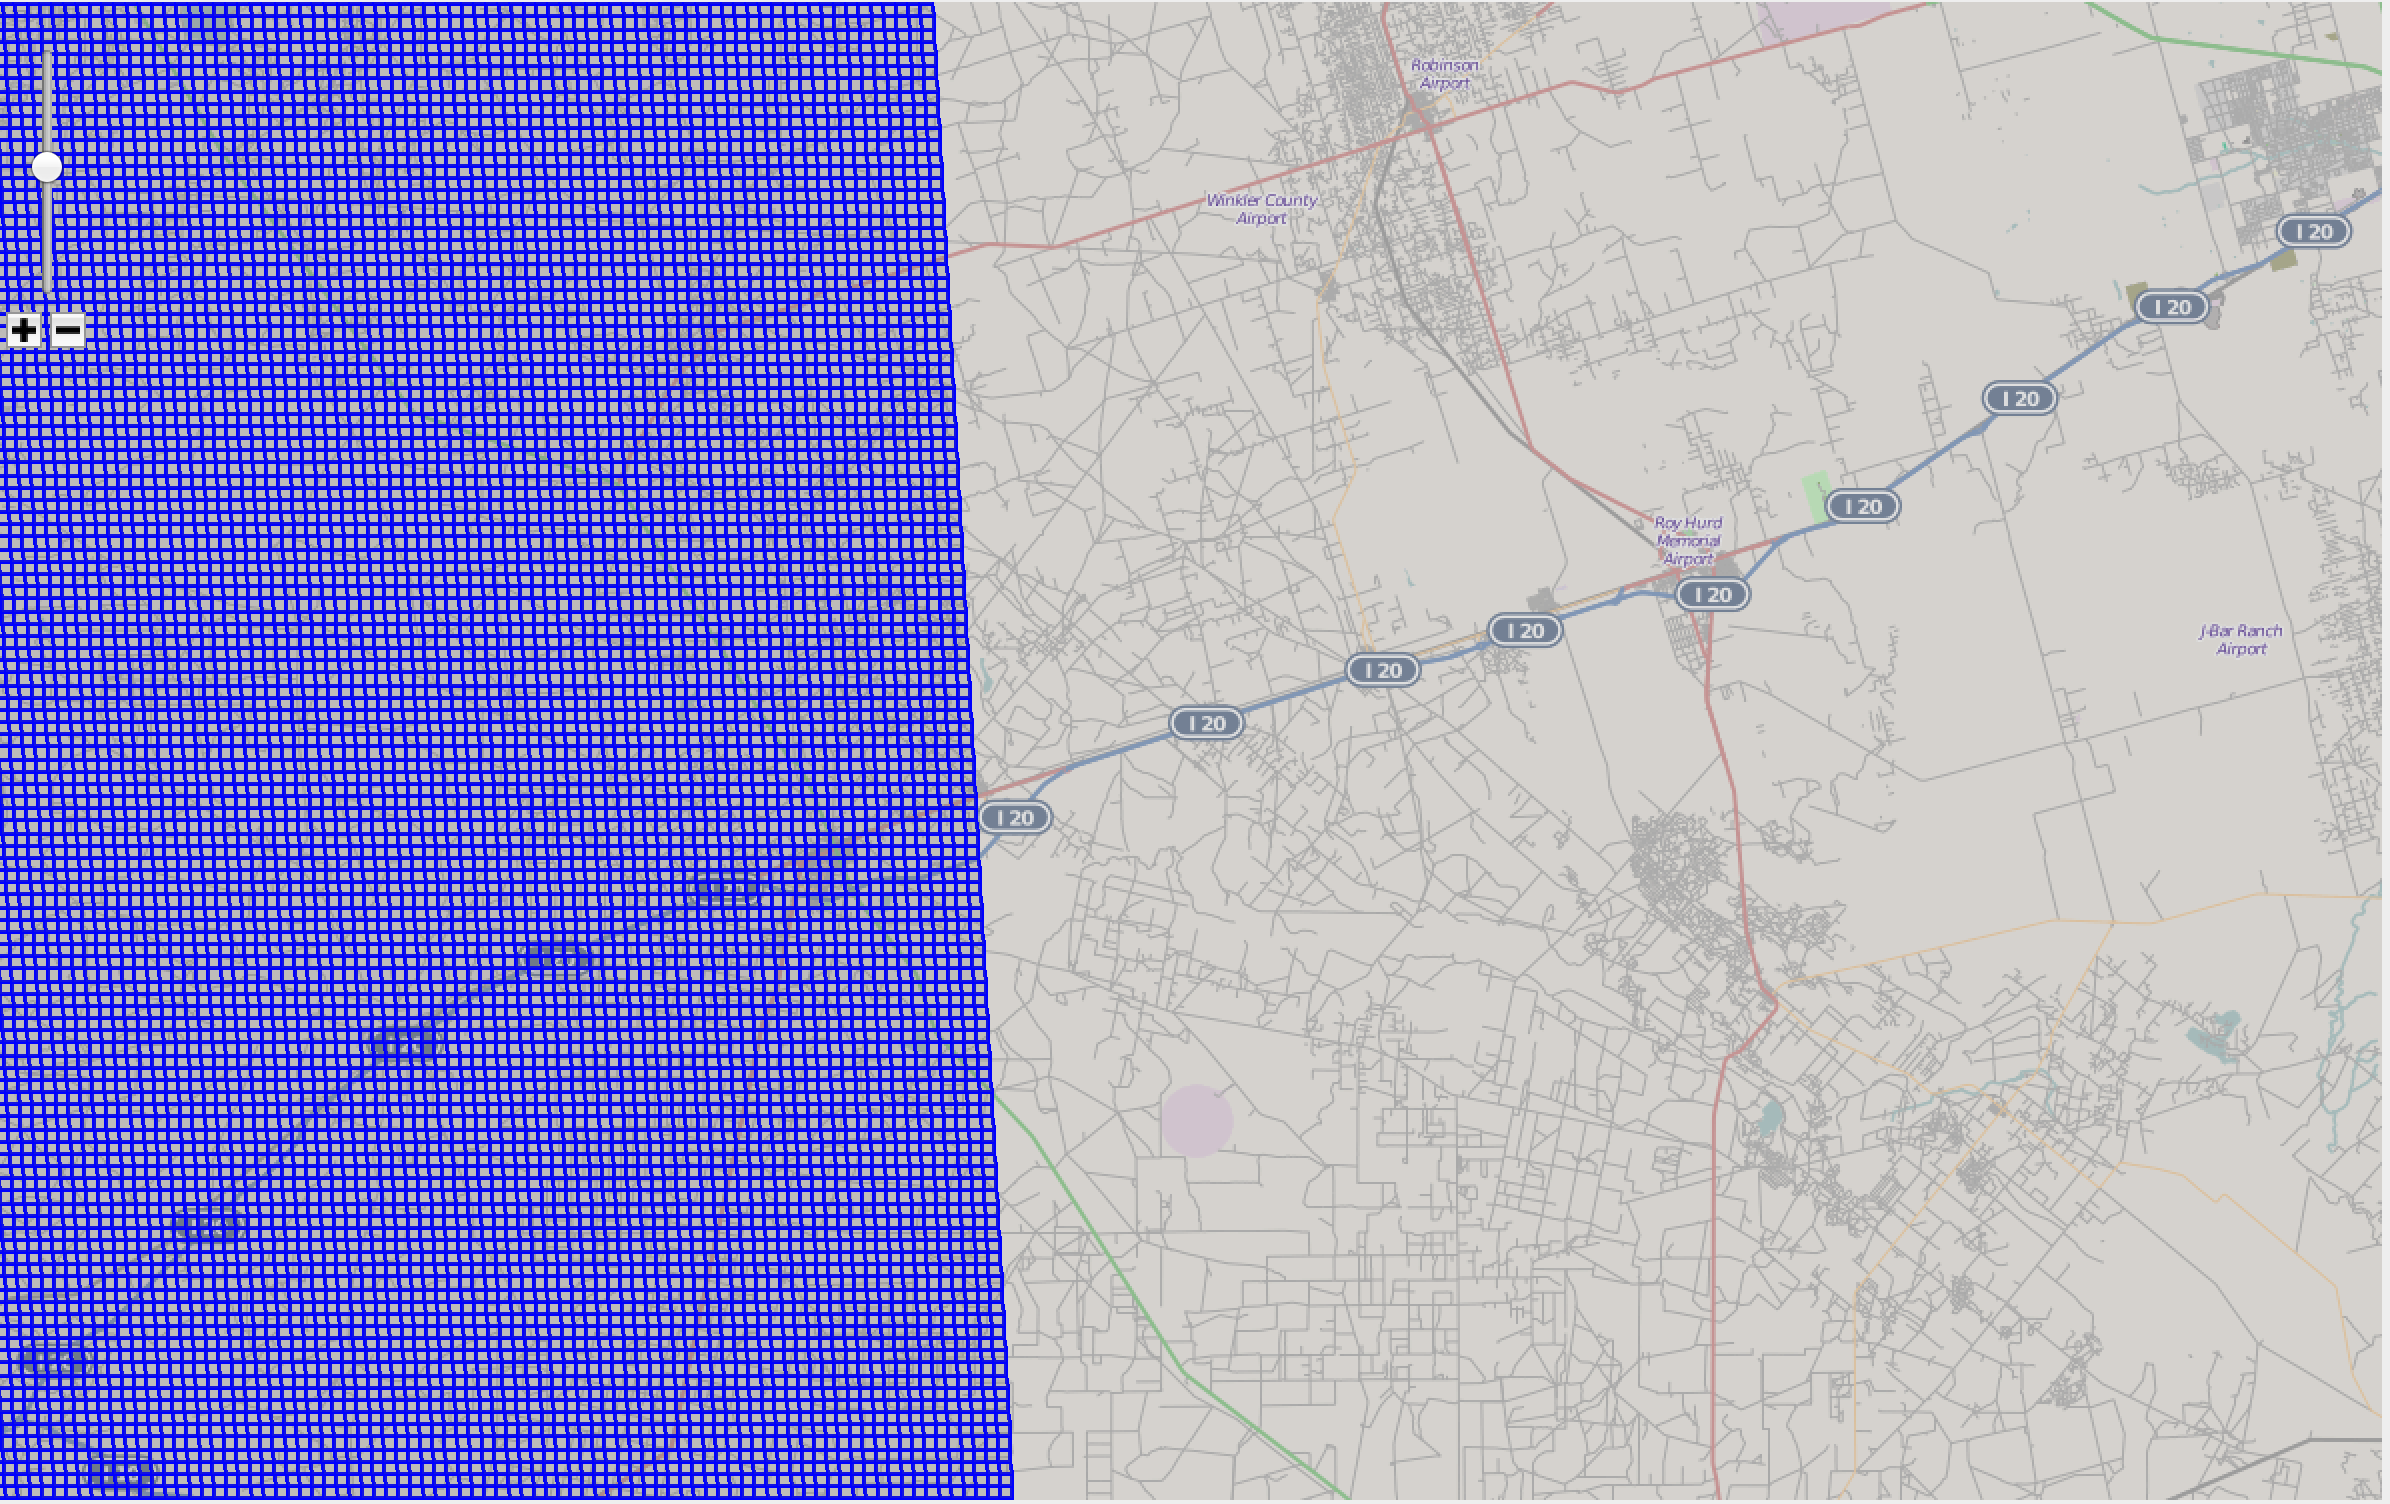
\includegraphics[width=0.8\textwidth]{./Figures/texasGrid.png}
\caption{The grid displayed on our OSM interface in TExas}
\label{fig:texasGrid}
\end{center}
\end{figure}

When zoomed, the properties of the grid is displayed. The pixels are increasingly non-square as one moves away from the (0,0) pixel.

\begin{figure}[t]
\begin{center}
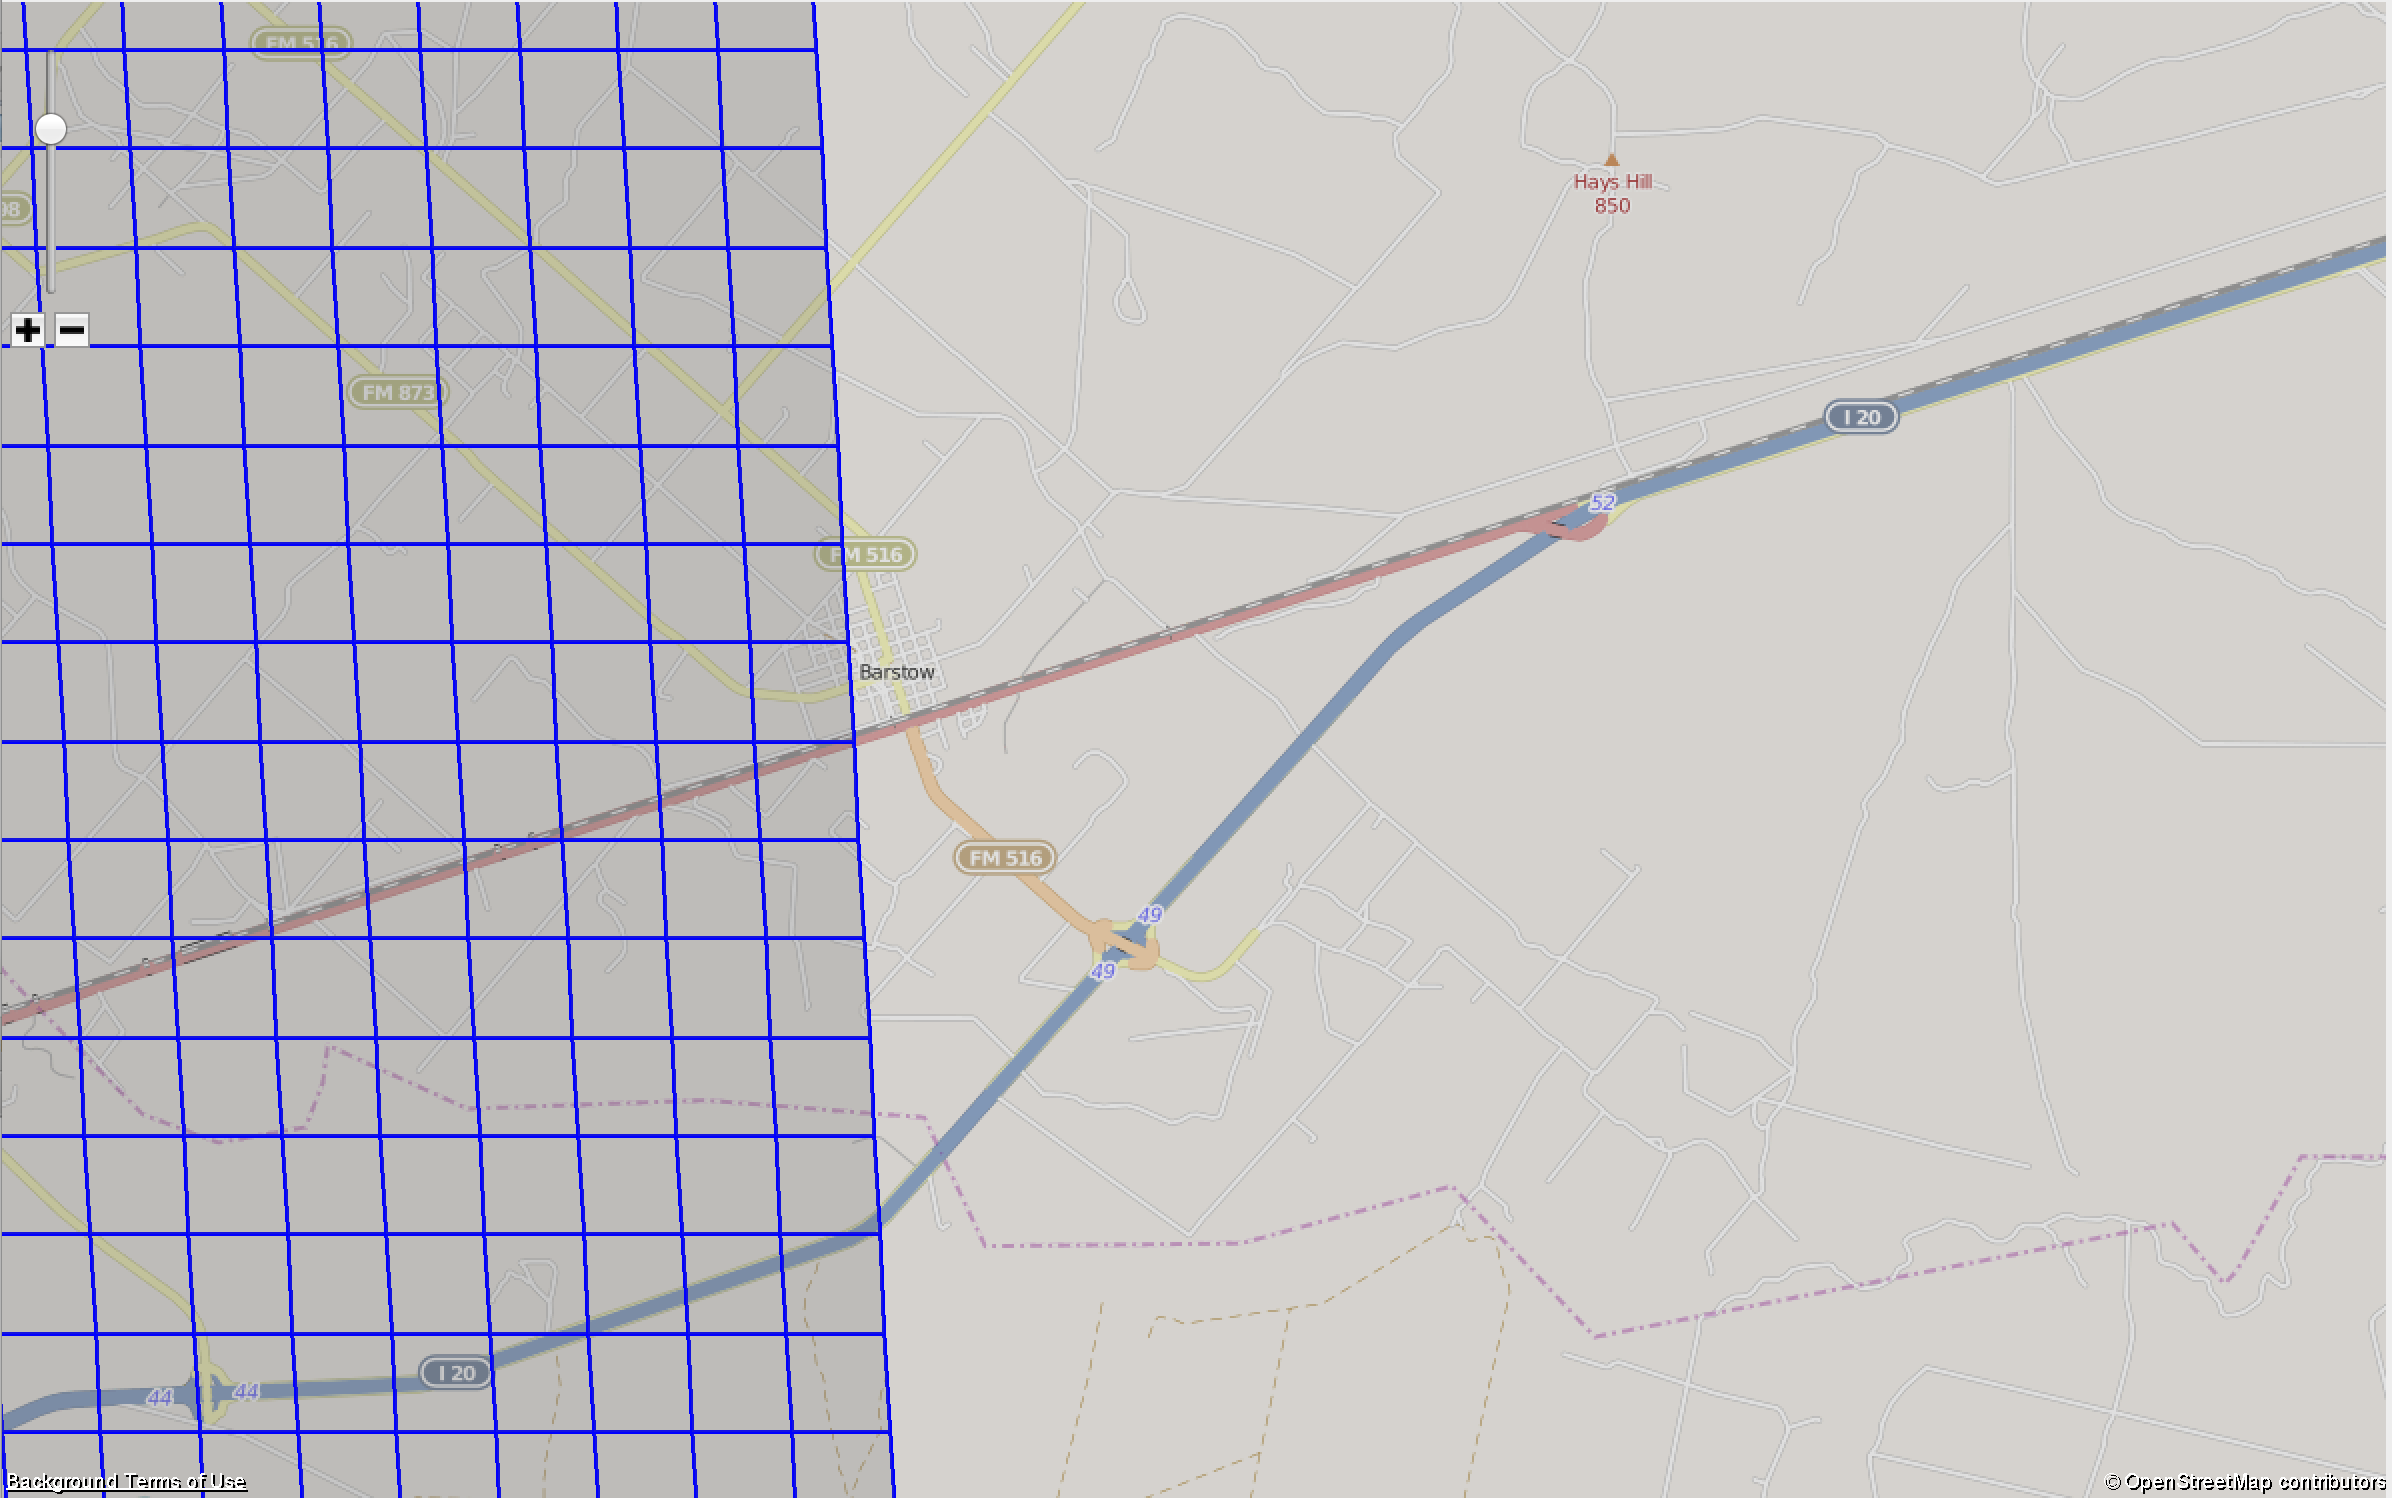
\includegraphics[width=0.8\textwidth]{./Figures/texasGridZoom.png}
\caption{The grid displayed on our OSM interface in Texas zoomed in}
\label{fig:texasGridZoom}
\end{center}
\end{figure}







